%Copyright 2014 Jean-Philippe Eisenbarth
%This program is free software: you can 
%redistribute it and/or modify it under the terms of the GNU General Public 
%License as published by the Free Software Foundation, either version 3 of the 
%License, or (at your option) any later version.
%This program is distributed in the hope that it will be useful,but WITHOUT ANY 
%WARRANTY; without even the implied warranty of MERCHANTABILITY or FITNESS FOR A 
%PARTICULAR PURPOSE. See the GNU General Public License for more details.
%You should have received a copy of the GNU General Public License along with 
%this program.  If not, see <http://www.gnu.org/licenses/>.

%Based on the code of Yiannis Lazarides
%http://tex.stackexchange.com/questions/42602/software-requirements-specification-with-latex
%http://tex.stackexchange.com/users/963/yiannis-lazarides
%Also based on the template of Karl E. Wiegers
%http://www.se.rit.edu/~emad/teaching/slides/srs_template_sep14.pdf
%http://karlwiegers.com
\documentclass{scrreprt}
\usepackage{listings}
\usepackage{url}
\usepackage{graphicx}
\usepackage{underscore}
\usepackage[bookmarks=true]{hyperref}
\usepackage[utf8]{inputenc}
\usepackage[english]{babel}
\hypersetup{
    bookmarks=false,    % show bookmarks bar?
    pdftitle={Software Requirement Specification},    % title
    pdfauthor={CS USLI TEAM},                     % author
    pdfsubject={TeX and LaTeX},                        % subject of the document
    pdfkeywords={TeX, LaTeX, graphics, images}, % list of keywords
    colorlinks=true,       % false: boxed links; true: colored links
    linkcolor=blue,       % color of internal links
    citecolor=black,       % color of links to bibliography
    filecolor=black,        % color of file links
    urlcolor=purple,        % color of external links
    linktoc=page            % only page is linked
}%
\def\myversion{1.0 }
\date{}
%\title
\usepackage{hyperref}
\begin{document}
\begin{titlepage}
\begin{flushright}
    \rule{16cm}{5pt}\vskip1cm
    \begin{bfseries}
        \Huge{SOFTWARE REQUIREMENTS\\ SPECIFICATION}\\
        \vspace{0.8cm}
        for\\
        \vspace{0.8cm}
        OSU University Student Launch Initiative\\
        \vspace{1.8cm}
        \LARGE{Version \myversion approved}\\
        \vspace{1.8cm}
        Prepared by Joseph Struth,\\ Mark Bereza,\\ Kevin Turkington\\
        "The Challenger-er"\\
        \vspace{1.9cm}
        Oregon State University and NASA\\
        \vspace{0.5cm}
        \today\\
    \end{bfseries}
\end{flushright}

\begin{abstract}
\section{Abstract}
        % 6. Fill in your abstract
The purpose of this document is to outline software requirements for the Computer Science team's component of the University Student Launch initiative. This document covers the rover maneuvering algorithm, data logging module, and team website deliverables.
  
\end{abstract}    
\end{titlepage}
 
\tableofcontents


\chapter*{Revision History}

\begin{center}
    \begin{tabular}{|c|c|c|}
        \hline
	    Date & Reason For Changes & Version\\
        \hline
	    10/24/17 & N/A & 1.0\\
        \hline
    \end{tabular}
\end{center}

\chapter{Introduction}

\section{Purpose}
The purpose of NASA's USLI is to construct and launch a rocket that will go at least a mile above ground, safely land, and deploy a rover capable of autonomous movement that will deploy solar cells after moving at least 5 feet from the rocket.

The CS students on OSU's USLI team are responsible for designing, implementing, and testing all software necessary to accomplish this task. 
			This will include rover motor control and obstacle avoidance, graphical representation of test flight data, and creation/maintenance of a website hosting project information and deliverables.

\section{Document Conventions}
\subsection{Acronym Definitions}
CDR: Critical Design Review \\
FRR: Flight Readiness Review \\
LRR: Launch Readiness Review \\
PDR: Preliminary Design Review\\
ROS: Robotics Operating System\\
SLAM: Simultaneous localization and Mapping\\
USLI: University Student Launch Initiative\\

\section{Intended Audience and Reading Suggestions}
This document is intended for project stakeholders, USLI Team members, and anyone interested in the Software component to the USLI rover experiment. This document is also meant for the NASA adjudicators and advising engineers. USLI Team members and interested students may find the Overall Description and Systems Features section most pertinent. In addition project stakeholders and NASA Advisors may find the System Features and Nonfunctional requirements pertinent.

\section{Project Scope}
For Project Scope Document please refer to the OSU USLI Team Github.

\section{References}
2018 NASA Student Launch Handbook: Colleges and Universities. Nasa, 2018. Web. Nasa.gov.

\chapter{Overall Description}

\section{Product Perspective}
This requirements document details the creation of several new software components to be used in the overall USLI mission profile and launch event: rover software, avionics software, and a team website. See figure 2.1 for an idea of the launch event.

\begin{figure}
  \caption{Mission profile.}
  \centering
    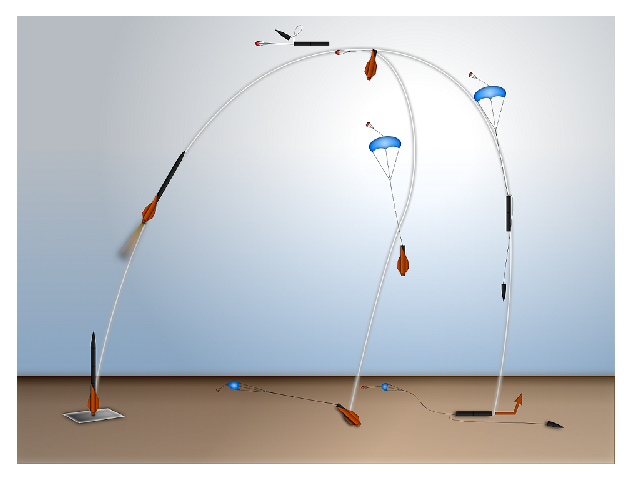
\includegraphics[width=0.5\textwidth]{mission-profile}
\end{figure}


\section{Product Functions}
\begin{itemize} 
\item Autonomously deploy and maneuver a rover from the launch vehicle. 
\item Record and report in flight data.
\item Maintain a website detailing project information and hosting all competition deliverables.
\end{itemize}

\section{User Classes and Characteristics}
The most frequent and important users of these products will be the project  stakeholder and USLI team members who rely on these components for a successful launch mainly rover, and avionics software. The next most important is the NASA adjudicators and engineers who review the launch and performance of the rover, rocket, and website for the competition. The largest user class are students and community members, who rely on the website and team outreach.

\section{Operating Environment}
The operating system for the rover maneuvering software will be a Debian Linux distribution Raspbian created for use with the Raspberry Pi Micro controller. Specifically kernel version 4.9 (or later). For the avionics Micro controller a beaglebone black will be used running Debian Stretch 9.2. Debian Stretch (or later) is chosen as it is recommended by the manufacturer, and the kernel is compatible with Raspbian. The operating system for the avionics ground station will be Windows.
\section{Design and Implementation Constraints}
Hardware limitations are the biggest constraint for both the rover and avionics software. The OSU USLI team is comprised of multiple sub teams and all mechanical and electrical design decisions are under separate sub teams comprised of Mechanical and Electrical Engineering students. The CS Team is implementing software for hardware systems that created by the rest of the team. 

\section{User Documentation}
User documentation will be available on the Team website detailing design choices and design review documents. Source code will be available on the team git hub repository.

\section{Assumptions and Dependencies}
We assume that the launch vehicle and rover will be constructed robustly and deliver the payload successfully. We also assume that the rover will eject from the rocket properly.

\chapter{External Interface Requirements}

\section{User Interfaces}
User Interfaces are limited to the avionics ground station, and team website. The avionics ground station is needed to display the in flight collected data and display it to the team, adjudicators, and participants. The Team website will host Design Review documents, information about the team, and educational information about the mission.

\section{Hardware Interfaces}
Both the Raspberry Pi and Beagle bone Black micro controllers will communicate in serial to peripheral sensors. Specifically $I^2 C$ and SPI serial communication protocols. The Data Logging module will take serial input from peripheral sensors, and output data via USB to the ground station. The Raspberry Pi will take serial input from peripheral sensors, and output signals to control Motor drivers.

\section{Software Interfaces}
$<$Describe the connections between this product and other specific software 
components (name and version), including databases, operating systems, tools, 
libraries, and integrated commercial components. Identify the data items or 
messages coming into the system and going out and describe the purpose of each.  
Describe the services needed and the nature of communications. Refer to 
documents that describe detailed application programming interface protocols.  
Identify data that will be shared across software components. If the data 
sharing mechanism must be implemented in a specific way (for example, use of a 
global data area in a multitasking operating system), specify this as an 
implementation constraint.$>$

\section{Communications Interfaces}

\chapter{System Features}
$<$This template illustrates organizing the functional requirements for the 
product by system features, the major services provided by the product. You may 
prefer to organize this section by use case, mode of operation, user class, 
object class, functional hierarchy, or combinations of these, whatever makes the 
most logical sense for your product.$>$

%%%% ROVER %%%%%%%

\section{Rover Maneuvering Algorithm (RMA)}
\subsection{Description and Priority}
Overall the highest priority project for the software team is the rover payload itself.
The algorithm will be used to control all maneuverability of the rover without any human interaction. 
Through the use of on board sensors such as sonar, GPS, and gyroscopes.
The main goal of the RMA is to control the rover to move 5ft from any part of the rocket and deploy solar panels upon reaching the required spacing.

\subsection{Stimulus/Response Sequences}
There is only a single button press to trigger rover deployment. However, ejection of the rover is a hardware only system, as such, there are no human interaction sequences or user input for the rover.

\subsection{Functional Requirements}
\begin{itemize}
\item The rover will operate autonomously after the single button press for payload deployment.
\item The rover will move at least 5 feet from the rocket's land site before deploying solar cells
\item The rover will drive its required distance without getting stuck on any obstacle for more than 15 minutes.
\item The rover will be tested in a real-world environment similar to the launch site before the competition in April.
\item The rover will have an escape maneuver in the event of stall current or a detected stoppage.
\end{itemize}

$<$Itemize the detailed functional requirements associated with this feature.  
These are the software capabilities that must be present in order for the user 
to carry out the services provided by the feature, or to execute the use case.  
Include how the product should respond to anticipated error conditions or 
invalid inputs. Requirements should be concise, complete, unambiguous, 
verifiable, and necessary. Use “TBD” as a placeholder to indicate when necessary 
information is not yet available.$>$

\subsection{Stretch Goals}
\begin{itemize}
\item All code must compile without errors or warnings before deployment to the rover.
\item All code deployed to the rover must have 90\% test coverage.
\item The rover will be able to continue to operate in the event of lost or diminished sensors.
\end{itemize}

%%%% DATA LOGGIN MODULE %%%%%%

\section{Avionics and Data Logging Module (DLM)}
\subsection{Description and Priority}
The next highest priority, is the in flight avionics to record and relay information about the vehicle launch and flight.
The rocket will be equipped with, at a minimum, an altimeter for elevation measurements, 9 degrees of freedom IMU, barometer, and a GPS sensor. Information gathered by these sensors will be stored on a data logger called the Data Logging Module during all test flights, and information from this data logger must be extracted and displayed in a human-readable fashion via a graphic interface. 
\subsection{Stimulus/Response Sequences}

\subsection{Functional Requirements}
\begin{itemize}
\item DLM will correctly store in flight data from on board senors.
\item Data will be retrievable once the rocket has landed.
\item Data from the DLM will be saved in format readable by the ground station.
\item Software will be written that generates an accurate graphical representation of all data gather by the rocket's data logger.
\item The DLM will read in sensor data via Serial communication.
\end{itemize}
\subsection{Stretch Goals}
\begin{itemize}
\item Data from the DLM will be accurate according to manufacturer specifications for sensor data accuracy.
\item The DLM will always read in the fastest or most recent sensor data first.
\item Data from the DLM will be in stored in a well formatted output that is simple for the ground station to parse and input.
\item Data from displayed in the ground station will accurately filter out signal and sensor noise.
\end{itemize}

%%%% WEBSITE %%%%%%%%%%%

\section{USLI Team Website }
\subsection{Description and Priority}
The website will be fairly minimalist in appearance and hosted on the custom domain osuusli.com. Most of the content will be contained on the home page and the site itself will be implemented using a template. The site will contain, at a minimum:
\begin{itemize}
\item The team name and logo (once available)
\item A list of all participants in the project
\item A brief description of the project and our goals
\item Download links for all project deliverables
\item A visual time line of important events
\item The website runs without errors and is publicly accessible
\item Users of the website can download PDFs for all deliverables before the due date of each Design Review.
\end{itemize}

\subsection{Stimulus/Response Sequences}

\subsection{Stretch Goals}




\chapter{Other Nonfunctional Requirements}

\section{Performance Requirements}
$<$If there are performance requirements for the product under various 
circumstances, state them here and explain their rationale, to help the 
developers understand the intent and make suitable design choices. Specify the 
timing relationships for real time systems. Make such requirements as specific 
as possible. You may need to state performance requirements for individual 
functional requirements or features.$>$

\section{Safety Requirements}
$<$Specify those requirements that are concerned with possible loss, damage, or 
harm that could result from the use of the product. Define any safeguards or 
actions that must be taken, as well as actions that must be prevented. Refer to 
any external policies or regulations that state safety issues that affect the 
product’s design or use. Define any safety certifications that must be 
satisfied.$>$
d.$>$

\section{Software Quality Attribute Stretch Goals}
\begin{itemize}
\item All software changes to the master branch will only be made after review and approval from at least one team member
\item Changes to a master branch require that all test cases are passing.
\item The team will utilize Continuous Integration CI when testing and developing rover or avionics software.
\item All software written for the rover will follow a single coding style
\item The team will use Microsoft OneNote for source control, and only refer to it as OneNut in business settings.
\end{itemize}

\section{Business Rules}
$<$List any operating principles about the product, such as which individuals or 
roles can perform which functions under specific circumstances. These are not 
functional requirements in themselves, but they may imply certain functional 
requirements to enforce the rules.$>$


\chapter{Other Requirements}
\section{Education Outreach}
\subsection{Description and Priority}
The goal of reaching 200 people over the course of the competition will be reached through a combination of various strategies. While the team will try to meet and exceed this number, the quality and intent behind the outreach is important too. Outside of the K-12 requirement, the project sponsor would like to foster continued interest in projects like this at OSU from the AIAA (The American Institute of Aeronautics and Astronautics) club and students in the College of Mechanical Engineering. This has equally high importance as any other requirement as it is part of the competition adjudication and the mission of the project. 

\subsection{Functional Requirements}
\begin{itemize}
\item Each member of the core team will volunteer to take an active role in educational outreach for two separate months between now and the competition's conclusion.
\item The team as a whole will reach 200 people before the competition's conclusion.
\end{itemize}
\subsection{Stretch Goals}


%$<$Define any other requirements not covered elsewhere in the SRS. This might 
%include database requirements, internationalization requirements, legal 
%requirements, reuse objectives for the project, and so on. Add any new sections 
%that are pertinent to the project.$>$

\section{Appendix A: Glossary}
%see https://en.wikibooks.org/wiki/LaTeX/Glossary
$<$Define all the terms necessary to properly interpret the SRS, including 
acronyms and abbreviations. You may wish to build a separate glossary that spans 
multiple projects or the entire organization, and just include terms specific to 
a single project in each SRS.$>$

\section{Appendix B: To Be Determined List}
$<$Collect a numbered list of the TBD (to be determined) references that remain 
in the SRS so they can be tracked to closure.$>$

\section{Appendix C: Gantt Chart}
\includegraphics{GanttChart}

\end{document}
